\documentclass[../main/main.tex]{subfiles}

\begin{document}

\section{Overview of exercises (PART I)}

\begin{enumerate}
\item limb-darkening scattering exercise we did during the course. 
— You can look into your notes from that, and I attach here also a sample program which you can use a base. After you have familiarised yourself with this, you can start to think bout how you would go about to extend this to a 3D setting (assuming isotropic scattering). 

\item (As prep for Monte-Carlo school) here is a script computing a UV resonance P-Cygni line in spherically symmetric wind with v beta-law. At top of routine, a few exercises are given, where you can modify and play around with code. Monte-Carlo program which computes a UV resonance spectral line from a fast outflowing spherically symmetric stellar wind (if you were not cc’d on that email, let me know so that I can send you the files as well). At the top of that little script, there are a few suggestions for exercises (additions) you could do to that program, in order to learn a bit more about the general workings of Monte-Carlo radiative transfer in this context.  
— So that might be a good idea for you to do as well !   (And you can also ask the others in the group for some tips etc. then.) 

\item Some background reading: 
\begin{itemize}
\item Attached mc manual by Puls. 
\item Paper by Sundqvist+ 2010 (Appendix, I think). 
\end{itemize}
\end{enumerate}


\section{Overview of exercises (PART II)}
\label{Overview_Part_2}

\begin{enumerate}
\item Calculate the probability distribution to sample from in the case of Eddington limb darkening for the initial distribution (see Section \underline{\ref{Eddington_limb_darkening_adaptation}}).
\begin{itemize}
\item finished + Ok
\end{itemize}

\item Calculate analytical solution for simplified problem in the case that \texttt{mu = 1} (see Section \underline{\ref{PCYG FIRST adaptation}}).
\begin{itemize}
\item finished + Ok + can be further studied
\end{itemize}

\item Perform convergence analysis (see Section \underline{\ref{convergence_analysis}}).
\end{enumerate}

\section{Overview of exercises (PART III)}
\label{Overview_Part_3}

\begin{enumerate}
\item Revisit 3D limb darkening. $\phi$ should be sampled between $0$ and $2\pi$ (see Section \underline{\ref{3D_limb_darkening}}). (OK)

\item Revisit convergence analysis: adapt plot formatting and standard deviation is defined as square root of variance (see Section \underline{\ref{convergence_analysis}}).

\item Test variance reduction technique (see Section \underline{\ref{variance_reduction_experiment}}).   

\item Some general considerations about the definitiion of specific intensity (see Section \underline{\ref{specific_intensity}}). (OK)

\item For the Monte Carlo approximation of the diffusion equation, why do wo have $N \sim \tau$ for low optical depth $\tau \ll 1$ (see Section \underline{\ref{diffusion_Monte_Carlo_mean_free_path}}).

\item Revisit the radial streaming approximation in \texttt{pcyg.f90} for lower optical depth (e.g. \texttt{xk0=0.5}).
(see Section \underline{\ref{PCYG FIRST adaptation}}).

\item What happens when you add a line (e.g. \@ $x=0.5=a$)? How would you do that? (see Section \underline{\ref{second_line}}) 

\item Towards a mathematical description of the problem.
\end{enumerate}

\newpage
\section{Overview of exercises (PART IV)}
\begin{enumerate}
\item Convergence analysis: also fit a line through the points (see Section \underline{\ref{convergence_analysis}}). Formally, we write $V = CN^x$ and determine both $C$ and $X$ from experimental data. Correspondingly, $\log(V) = \log(C) + x\log(N)$. This is fitted using least-squares.

\item Variance reduction technique
\begin{itemize}
\item averaging over different stochastic realizations?
\item take \texttt{xk0=0.5}
\item try to also discretize $\mu$
\end{itemize}

\item Adding a second line: develop computer code in the radial streaming assumption (use analytic formulas) $\mu = 1$ (see Section \underline{\ref{two_resonance_lines}}).
\begin{itemize}
\item a following improvement is the use of a grid instead of using the bisection method.
\end{itemize}

\end{enumerate}


\newpage
\section{Limb darkening program}

\label{limb_darkening_discussion}

\subsubsection{2D Case}
We again have $\mu = \cos(\theta)$. The solution of the radiative transfer equation in \underline{plane-parallel syummetry} with frequency-independent absorption and emission, is 
\begin{equation}
I(\mu) = I_1 (0.4 + 0.6\mu)
\end{equation}
In the Monte Carlo code, the photons are sorted according to the direction that they leave the atmosphere.

\paragraph{Goal}
Calculates the angular dependence of photon's emitted from a plane-parallel, grey atmosphere of radial optical depth \texttt{taumax}. The value of \texttt{tau} determines the position of the photon

\paragraph{Variables and Algorithm}
\begin{itemize}
\item \texttt{muarray} contains emergent photons
\item \texttt{na} number of channels
\item \texttt{dmu} = 1/\texttt{na} width of channels
\item \texttt{nphot} number of photons
\item \texttt{taumax} maximum optical depth
\end{itemize}

\begin{algorithm}
\caption{Limb darkening: compute quantitiy of photons}\label{limb_darkening}
\begin{algorithmic}
\State initialization \\
\quad radial optical depth $\tau$ \\
\quad direction $\mu$

\For{all photons} 

\State $\boxed{\tau = \tau_{max}}$
	\While{\texttt{tau} $\geq 0$} 
	
	\State compute scattering angle \texttt{mu}
	\If{tau $\geq$ taumax} $\boxed{mu = sqrt(x)}$ (initial distribution)
	\Else{ $\boxed{mu = 2*x = 1}$} (isotropic scattering)
	\EndIf
	
	\State tau\_i = -log(x2) 
	\State tau = tau - tau\_i*mu	
		
	\EndWhile
	\State \textbf{end while}

	\State now we know that the photon has left the photosphere	
	\State compute the distribution of all angles \texttt{mu} at which the photon left the photosphere
	
\EndFor
\State \textbf{end for}

\State visualisation: 
	\begin{itemize}
	\item plot photon numbers from $\mu d\mu$ against \texttt{mu}
	\item plot specific intensity from $d\mu$ against \texttt{mu} against 
	\end{itemize}


\end{algorithmic}
\end{algorithm}


\begin{figure}[!htp]
\centering
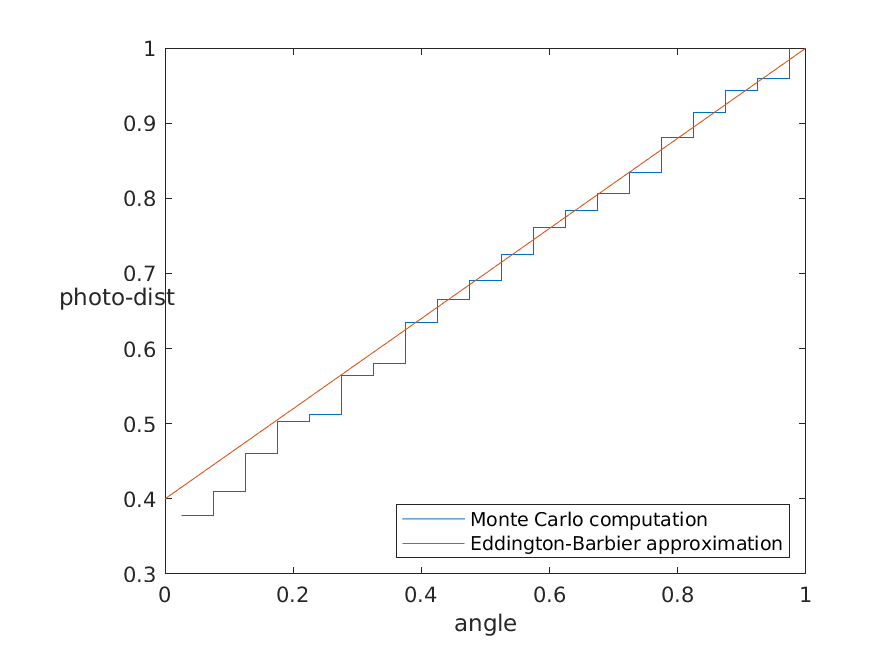
\includegraphics[width=0.7\textwidth]{../../introductory_exercises/limb_darkening/data/number_channels20number_photons100000max_opt_depth10.png}
\caption{histogram for \texttt{mu}}
\label{2D_mu}
\end{figure}
Figure \ref{2D_mu} is according to what is expected $I = I_0(0.4+0.6\mu)$. The input parameters are as follows \texttt{Limb\_Darkening(number\_of\_channels = 20, number\_of\_photons = $10^5$, \\ maximum\_optical\_depth = 10)}.

\newpage
\subsubsection{3D Code}
\label{3D_limb_darkening}

What changes is this: 
\begin{itemize}
\item introduction of a new angle $\phi$
\item the optical depth is not updated with respect to $\phi$ 
\end{itemize}


\begin{figure}[!htp]
\centering
\begin{minipage}{.5\textwidth}
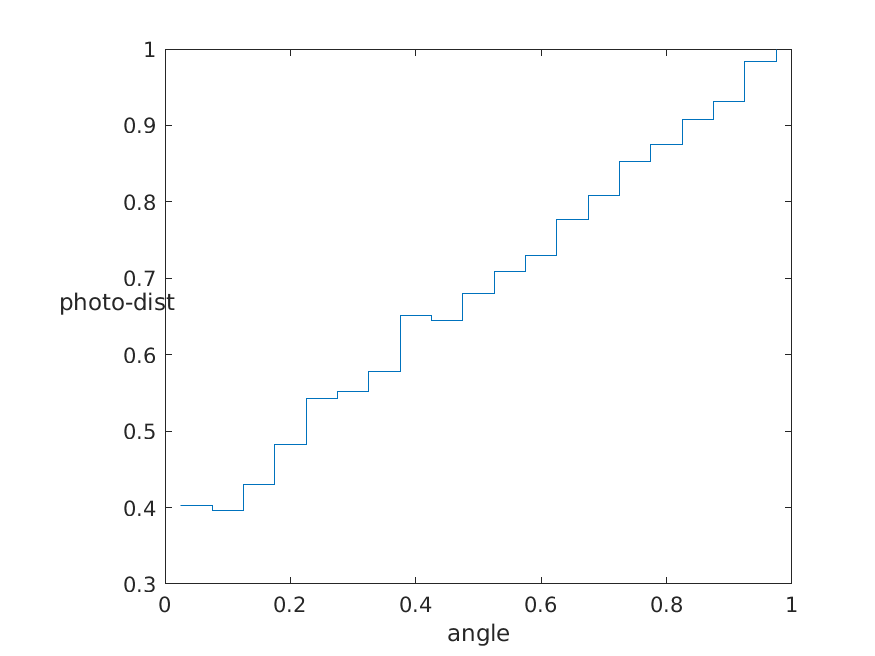
\includegraphics[width=\textwidth]{../../introductory_exercises/limb_darkening/data/LD_3D_mu_number_channels20number_photons100000max_opt_depth10.png}
\caption{histogram for \texttt{mu}}
\label{3D_mu}
\end{minipage}%
\begin{minipage}{.5\textwidth}
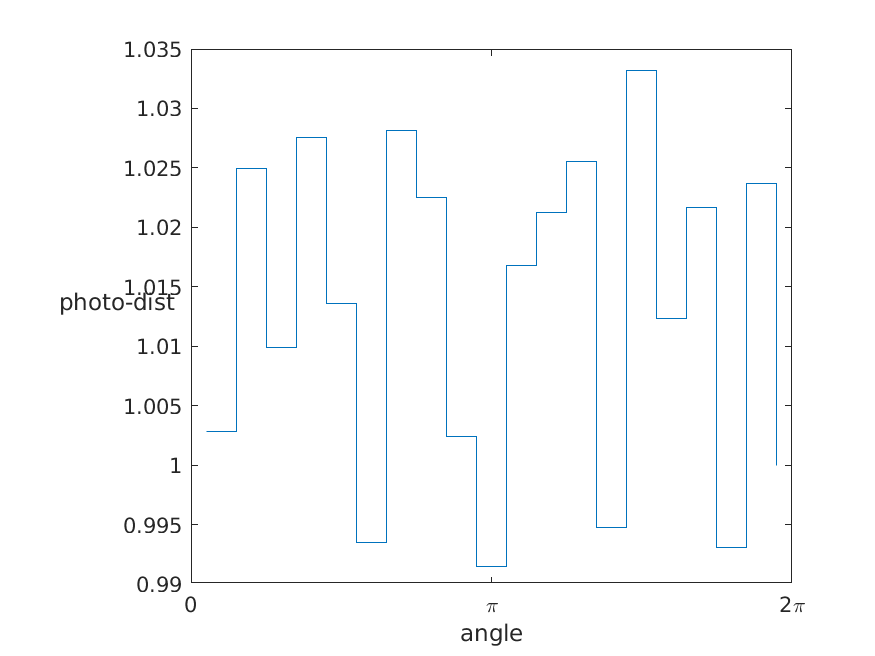
\includegraphics[width=\textwidth]{../../introductory_exercises/limb_darkening/data/LD_3D_phi_number_channels20number_photons100000max_opt_depth10.png}
\caption{histogram for \texttt{phi}}
\label{3D_phi}
\end{minipage}
\end{figure}

Figure \ref{3D_mu} and Figure \ref{3D_phi}  are the result of 
the function \texttt{Limb\_Darkening\_3D} with the following input parameters: \texttt{Limb\_Darkening\_3D(number\_of\_channels = 20, number\_of\_photons = $10^5$, \\ maximum\_optical\_depth = 10)}. The results according to what is expected, namely $I = I_0(0.4+0.6\mu)$ and $\phi$ follows a uniform distribution.

\paragraph{}
\noindent\fbox{
  \parbox{\textwidth}{
\textbf{Extension}: make version where the optical depth is updated with respect to $\phi$ 
}}

\vspace{0.4cm}
Via this link, you can go back to the exercises overview: Section \underline{\ref{Overview_Part_3}}.

\newpage
\section{Spectral line formation: pcyg.f90}
This section is about the study of line formation in an expanding wind.

\subsection{Overview of variables}
\begin{center}
\centering
{\tabulinesep=1.5mm
\begin{tabu}{|c|c|c|}
\hline 
name & explanation \\ \hline \hline

\multicolumn{2}{|c|}{\cellcolor{orange} paramaters} \\ \hline
xk0 & \\ \hline
alpha & velocity profile parameter \\ \hline
beta & velocity profile parameter \\ \hline \hline

\multicolumn{2}{|c|}{\cellcolor{orange} start frequency of the photon} \\ \hline
xstart & start frequency \\ \hline
vmin & \\ \hline
vmax  & \\ \hline

\multicolumn{2}{|c|}{\cellcolor{orange}angle of the photon} \\ \hline
xmuestart & start angle \\ \hline
xmuein & incident angle \\ \hline
xmueou & outward angle \\ \hline
\cellcolor{yellow} pstart & impact parameter \\ \hline
xnew & new photon frequency \\ \hline \hline

\multicolumn{2}{|c|}{\cellcolor{orange} optical depth} \\ \hline
tau & optical depth \\ \hline

\multicolumn{2}{|c|}{\cellcolor{orange} number of photons admin} \\ \hline
nphot & number of photons\\ \hline
nin & photons scattered back into core \\ \hline
nout & photons escaped \\ \hline \hline

\multicolumn{2}{|c|}{\cellcolor{orange} functions} \\ \hline
func & velocity profile \\ 
	& distance from center of star $r$ \\ \hline
	
xmueout & outwards (scattered) angle \\ 
& xk0 \\ 
& alpha \\ 
& r \\ 
& v \\ 
& sigma \\ \hline
\end{tabu}}
\end{center}

The amout of bins \texttt{nchan = 100}.


\newpage
\subsection{Mathematical things that are noteworthy}

\subsubsection{General working}
\begin{center}
\begin{tikzpicture}
[node distance=2.5cm,auto,>=latex']
    \node [int] (a) {\texttt{pcyg.f90}};
    \node (b) [left of=a,node distance=4cm, coordinate] {a};
    \node (c) [right of=a,node distance=4cm, coordinate] {a};
    \path[->] (b) edge node {\texttt{xstart}} (a);
    \path[->] (a) edge node {\texttt{xnew}} (c);
\end{tikzpicture}
\end{center}
The photons are sorted according to \texttt{xnew}.
In general, the flux is dependent on $\mu$ and the frequency $x$.


\begin{itemize}
\item I think that it satisfies $N(x)dx \sim I(x)xdx$
\item We are thus interested in $F_{\lambda} = F_{\nu}$
\end{itemize}


\subsubsection{Practical formula}
\begin{itemize}
\item emission angle $\mu = \cos(\theta)$
\item according p-ray $p = \sqrt{1-\mu^2} = \sin(\theta)$
\item incident angle $\texttt{xmuein} = \sqrt{1-\left(\frac{pstart}{r}\right)^2}$
\end{itemize}

\subsubsection{Geometry \& Symmetry assumptions}
\begin{itemize}
\item spherical geometry
\end{itemize}


\newpage
\subsection{Exercises}
\subsubsection{Investigation of original code}
In original version of the code, all photons are released isotropially from the photosphere.

\begin{figure}[!htp]
\centering
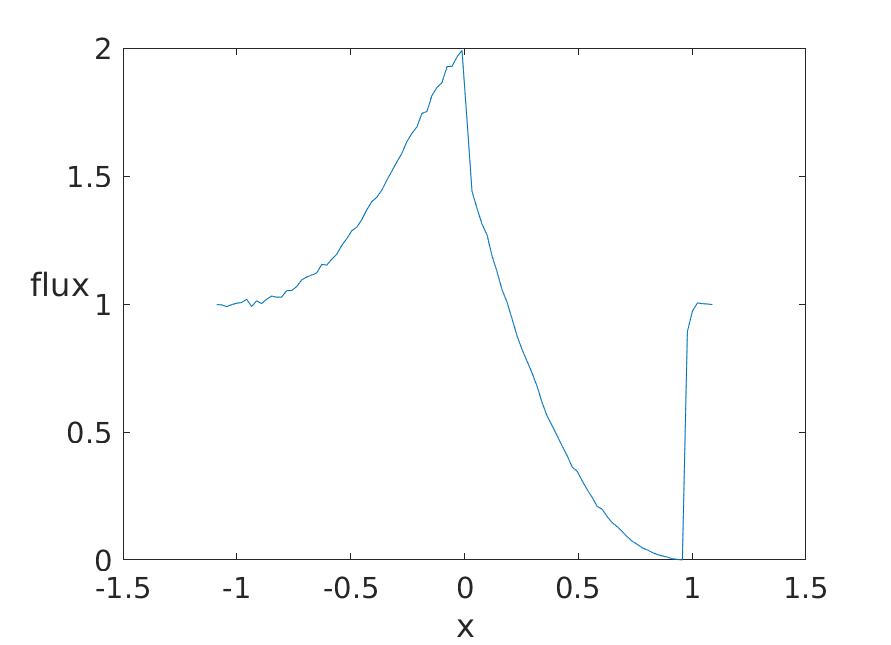
\includegraphics[width=0.5\textwidth]{../../introductory_exercises/P_Cygni_profile_UV_resonance/data/npot6xk0100alpha0beta1test0.png}
\caption{Original version of the code}
\end{figure}

\newpage
\subsubsection{First adaptation: what if all photons are released radially from photosphere?}
\label{PCYG FIRST adaptation}

\paragraph{\underline{Release photons radially: numerical MC experiments}}
What would happen with line-profile, if you assumed all photons
were released radially from photopshere?
\begin{itemize}
\item In other words $\texttt{xmuestart} = 1$. 
\item This is implemented under the test case \texttt{test\_number=1}.
\item Results in Figure \ref{PCyg_mu_eq_1} for opacity \texttt{xk0 = 100}.
\end{itemize}

\begin{figure}[!htbp]
\centering
\begin{subfigure}{.5\textwidth}
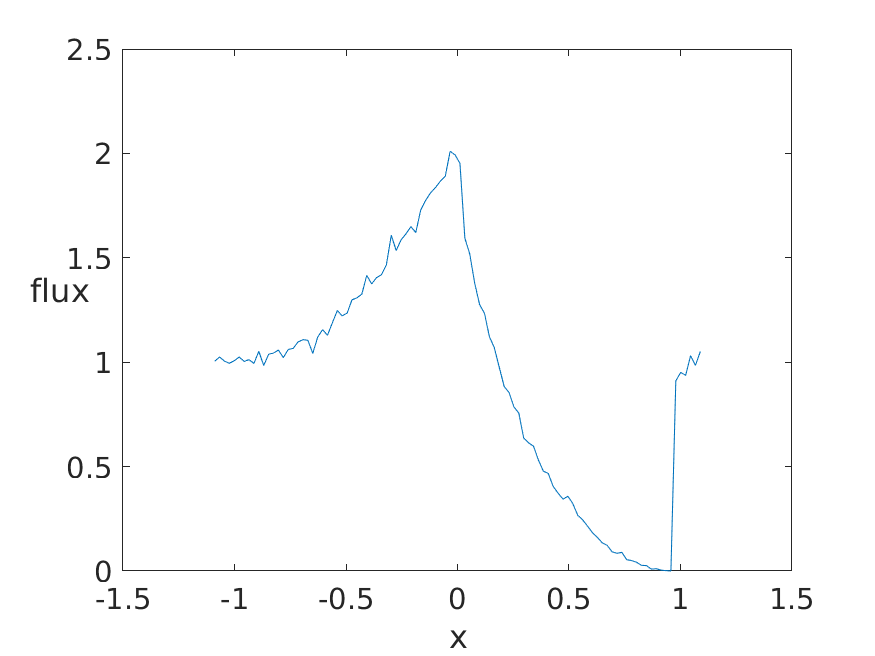
\includegraphics[width=1\textwidth]{../../introductory_exercises/P_Cygni_profile_UV_resonance/data/npot5xk0100alpha0beta1test1.png}
\caption{First adaptation}
\end{subfigure}%
\begin{subfigure}{.5\textwidth}
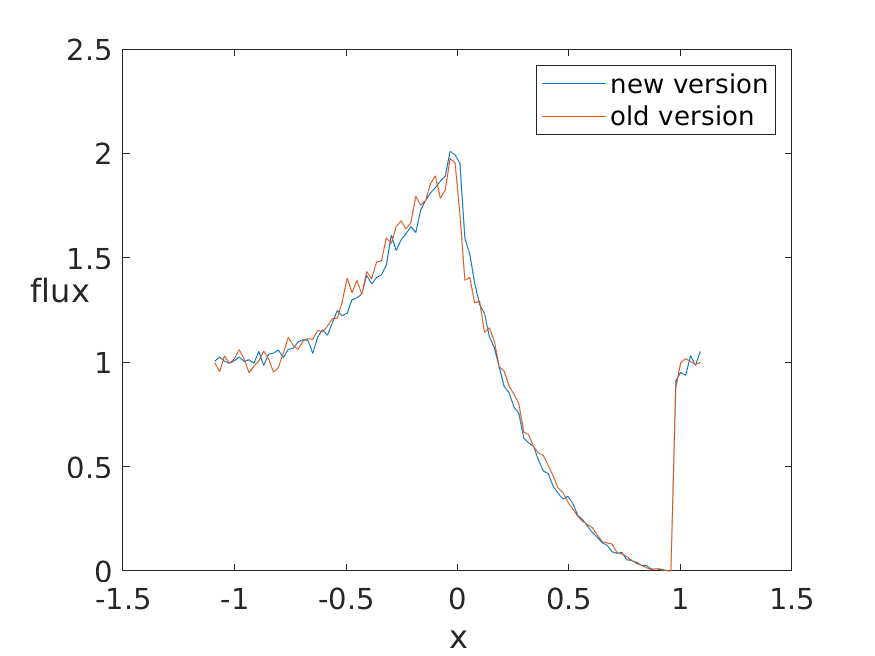
\includegraphics[width=1\textwidth]{../../introductory_exercises/P_Cygni_profile_UV_resonance/data/npot5xk0100alpha0beta1test10.png}
\caption{Same plot (together with output of initial version)}
\end{subfigure}
\caption{The number of photons equals $10^{5}$, \texttt{xk0=100}}
\label{PCyg_mu_eq_1}
\end{figure}


\paragraph{\underline{Derive analytic expression}} See also slide  26/49 [Sundqvist course material]. 
\begin{itemize}
\item since \texttt{xmuein = 1} we have for the velocity profile 
\begin{equation}
v = v_{\infty}(1-b/r)^{\beta}
\label{velocity_profile}
\end{equation}
A scaled version of Equation (\ref{velocity_profile}) yields 
\begin{equation}
u = \frac{v(r)}{v_{\infty}} = \left(1 - \frac{r_{\infty}}{r} \right)^{\beta} 
\label{u_profile}
\end{equation}
with $u \in [0..1]$

\item Doppler shift for the frequency of the photons: $x_{CMF} = x_{REF} - \mu u$.
\item Condition for resonance from Sobolov approximation (to be studied later): $\boxed{x_{CMF}= 0}$ thus 
\begin{equation}
x_{REF} = \mu u
\label{analytic_profile}
\end{equation}
or thus $x_{REF} = \boxed{u_{\text{interaction}}}$ and than solve Equation \ref{u_profile} for $r_{\text{interaction}}$


\item If $\mu = 1$ then 
\begin{equation}
x = \left(1 - \frac{r_{\infty}}{r} \right)^{\beta}
\end{equation}
\begin{equation*}
x^{1/\beta} = 1 - \frac{r_{\infty}}{r}
\end{equation*}
\begin{equation*}
r(1-x^{1/\beta}) = r_{\infty}
\end{equation*}
\begin{equation}
\boxed{r(x) = \frac{r_{\infty}}{1-x^{1/\beta}}}
\end{equation}

\noindent\fbox{
  \parbox{0.6\textwidth}{
  attention, here was something wrong! }} 

\item From the location of interaction $r$, the incident angle can be calculated
\begin{equation}
\texttt{xmuein} = \sqrt{1-\left[\frac{\texttt{pstart}}{r}\right]^2} = \sqrt{1 - \left[ \frac{\sqrt{1-\texttt{xmuestart}^2}}{r} \right]^2}
\end{equation}
Now also taking into account that \texttt{xmuestart = 1} then yields
\begin{equation}
\texttt{xmuein = 1}
\end{equation}

\item The calculation of the optical depth goes as follows:
\begin{equation}
\tau = \frac{\texttt{xkO}}{rv^{2-\alpha}(1+\texttt{xmuein}^2 \sigma)}
\end{equation}
Now also taking into account that \texttt{xmuestart = 1} gives
\begin{equation}
\tau = \frac{\texttt{xk0}}{rv^2(1+\sigma)}
\end{equation}

where $\boxed{v(x) = \left(1 - \frac{b}{r} \right)^{\beta}}$ 
\quad and $\frac{dv}{dr} = \frac{\beta b}{r^2}\left( 1 - \frac{b}{r} \right)^{\beta - 1}$  \\
and $\sigma(x) = \frac{dv}{dr}\frac{r}{v}-1$ 
thus $\boxed{\sigma(x) = \frac{\beta b}{r}\left( 1-\frac{b}{r}\right)^{-1}}$

\item Assuming that $\beta = 1$ then $\boxed{v(x) = 1 - \frac{b}{r}}$ and $\frac{dv}{dr} = \frac{\beta b}{r^2}$ and $\boxed{\sigma(x) = \frac{\beta b}{r}}$.

\item Conclusion: $\tau(x)$ is only dependent on $x$ and not on \texttt{xmuestart} or \texttt{xmuein}.

\item \texttt{xmueou} follows the distribution as given by the function \texttt{xmueout}, namely
\begin{equation}
p(x) = \frac{1-e^{-\tau}}{\tau}
\end{equation}
with $\tau = \frac{\texttt{tau0}}{1+\texttt{X}^2 \sigma}$ where $\texttt{X}$ is a random number, so actually this comes down to
\begin{equation}
\boxed{p(x) = \frac{1-e^{-\frac{\tau_0}{1+x^2\sigma(x)}}}{\frac{\tau_0}{1+x^ 2\sigma(x)}}}
\end{equation}

\item Finally one can combine these results to get the distribution of the photons according to the frequency $x$ via the relation 
\begin{equation}
\texttt{xnew = xstart + v(xmueou-xmuein) = xstart + v(xmueou -1)}
\label{pcyg_mu_1_final_eq}
\end{equation}

In words, we initially have an isotropic distribution for \texttt{xstart}. The number of photons that are leaving the atmosphere at different frequencies is however not isotropic through complex interactions that are incorporated into $p(x)$.
One must also take into account that not all of the photons that are released actually escape from the atmosphere and also that sometimes no resonance is possible, and then Equation (\ref{pcyg_mu_1_final_eq}) is not applicable.

\end{itemize}

\noindent\fbox{
  \parbox{\textwidth}{TO DO: proceed from this to the analytical expression for the flux. Here I am stuck for the moment.}}
  
\vspace{1cm}
Via this link, you can go back to the exercises overview: Section \underline{\ref{Overview_Part_2}.}

\newpage
\paragraph{\underline{Experiments with other opacities}}
The results for \texttt{xk0=0.5} are shown in Figures \ref{PCyg_mu_eq_1xk0_05} and \ref{PCyg_mu_eq_xk0_05_vs_100}.


\begin{figure}[!htbp]
\centering
\begin{subfigure}{.5\textwidth}
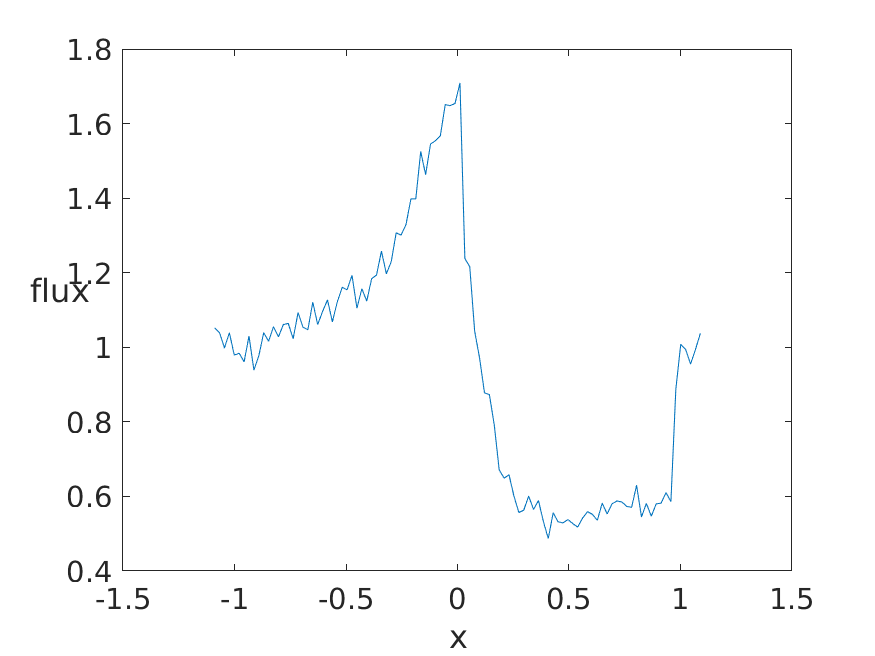
\includegraphics[width=1\textwidth]{../../introductory_exercises/P_Cygni_profile_UV_resonance/data/npot5xk05alpha0beta1test1.png}
\caption{First adaptation}
\end{subfigure}%
\begin{subfigure}{.5\textwidth}
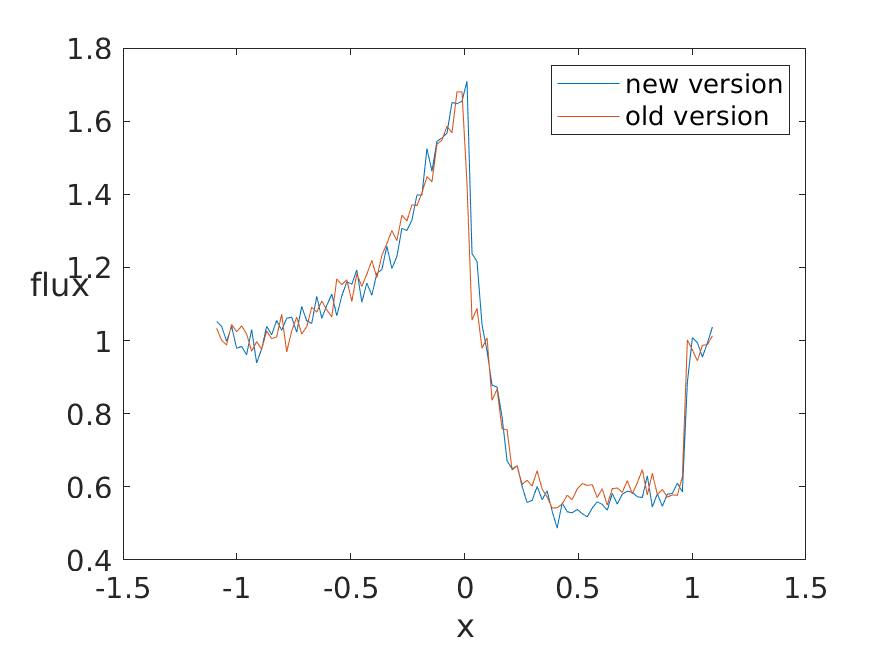
\includegraphics[width=1\textwidth]{../../introductory_exercises/P_Cygni_profile_UV_resonance/data/npot5xk05alpha0beta1test10.png}
\caption{Same plot (together with output of initial version)}
\end{subfigure}
\caption{The number of photons equals $10^{5}$, \texttt{xk0=0.5}}
\label{PCyg_mu_eq_1xk0_05}
\end{figure}

\begin{figure}[!htbp]
\centering
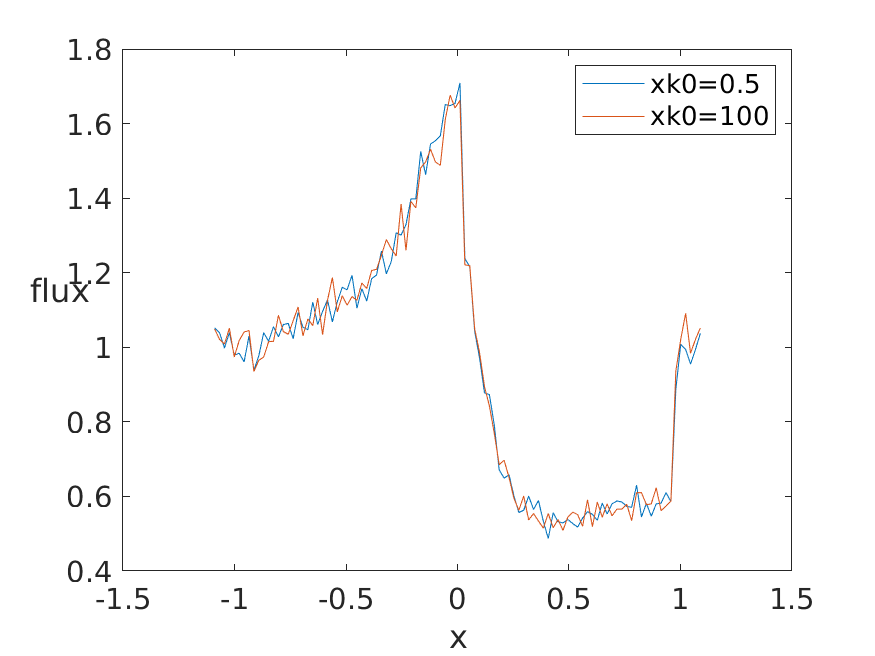
\includegraphics[width=0.5\textwidth]{../../introductory_exercises/P_Cygni_profile_UV_resonance/data/npot5xk05alpha0beta1test11.png}
\caption{The number of photons equals $10^{5}$, \texttt{xk0=0.5}}
\label{PCyg_mu_eq_xk0_05_vs_100}
\end{figure}

Via this link, you can go back to the exercises overview: Section \underline{\ref{Overview_Part_3}}.


\newpage
\subsubsection{Second adaptation: isotropic scattering}
\label{isotropic_scattering}
What would happen to line-profile, is you assumed scattering
was isotropic 
\\(i.e., NOT following Sobolev-distrobution)

\begin{itemize}
\item in the implementation, \texttt{test\_number = 2}
\item the results are shown in Figure \ref{Pcyg_isotropic_scattering}.
\end{itemize}


\begin{figure}[!htbp]
\centering
\begin{subfigure}{.5\textwidth}
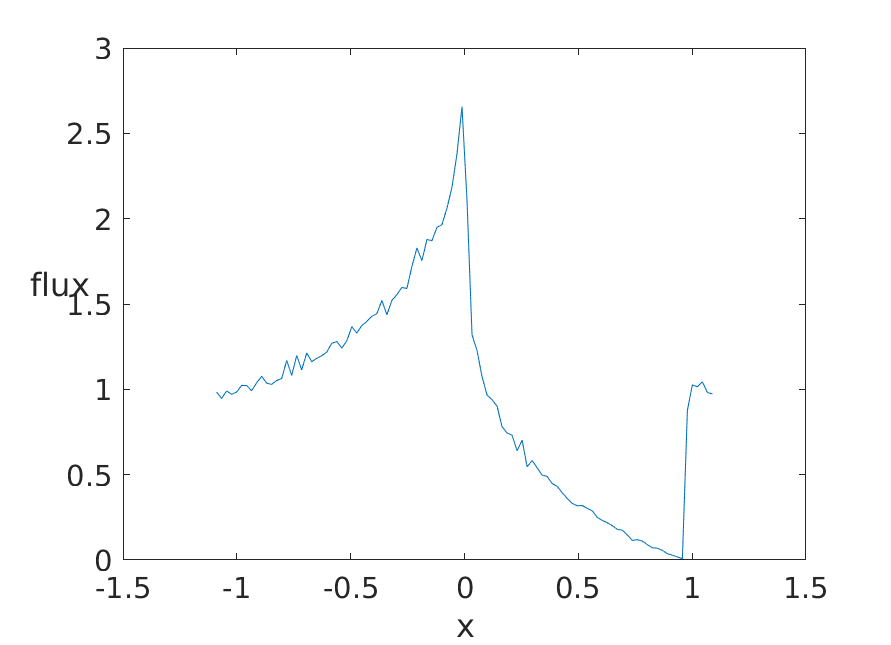
\includegraphics[width=1\textwidth]{../../introductory_exercises/P_Cygni_profile_UV_resonance/data/npot5xk0100alpha0beta1test2.png}
\caption{Second adaptation}
\end{subfigure}%
\begin{subfigure}{.5\textwidth}
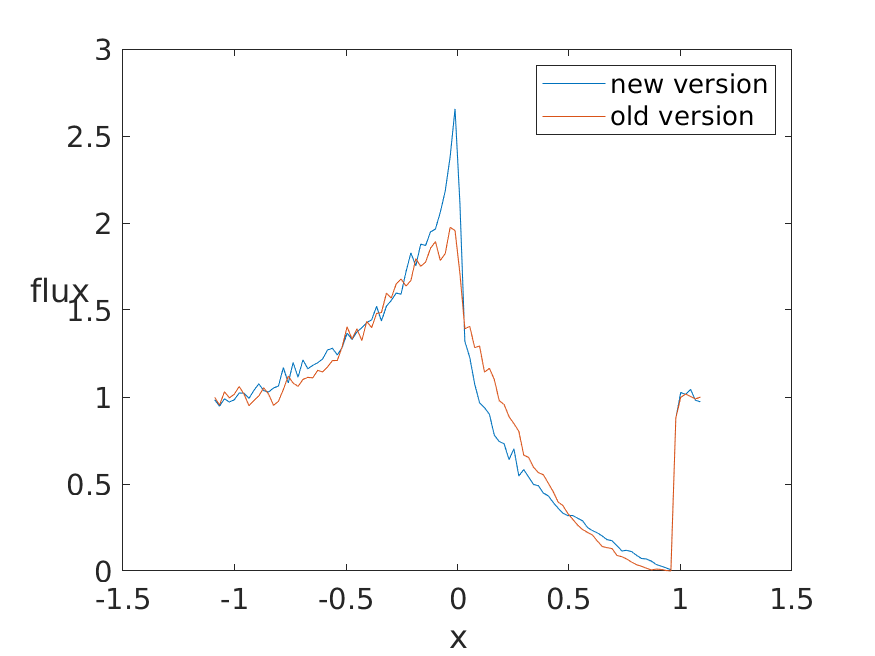
\includegraphics[width=1\textwidth]{../../introductory_exercises/P_Cygni_profile_UV_resonance/data/npot5xk0100alpha0beta1test20.png}
\caption{Same plot (together with output of initial version)}
\end{subfigure}
\caption{The number of photons equals $10^{5}$}
\label{Pcyg_isotropic_scattering}
\end{figure}

It is clear from Figure \ref{Pcyg_isotropic_scattering} that the peak around $x=0$ is higher and sharper. \\
\noindent\fbox{
  \parbox{0.35\textwidth}{Analyse this behaviour more closely}}

\newpage
\subsubsection{Third adaptation: introduction of Eddington limb-darkening}
\label{Eddington_limb_darkening_adaptation}
Put Eddington limb-darkening in. What happens? 

\paragraph{General (introductory) discussion: Eddington limb darkening}
The data are taken from Christensen, 2015.
\begin{itemize}
\item the source function $S= \braket{I} = a + b\tau_{\nu}$ with $a= \frac{\sigma}{2 \pi}T_{eff}^4$ and $b = \frac{3 \sigma}{4 \pi}T_{eff}^4$
\item solve the equation
\item this yields $\frac{I(\theta)}{I(0)} = \frac{a+b\cos(\theta)}{a+b} = \frac{2}{5} + \frac{3}{5}\cos(\theta)$
\end{itemize}

\begin{figure}[!htp]
\centering
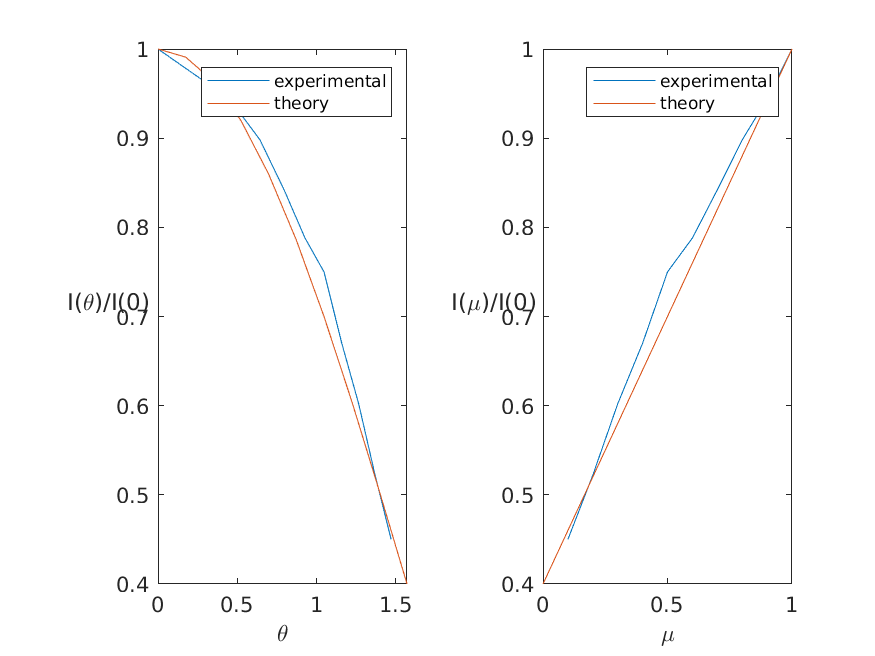
\includegraphics[width=0.7\textwidth]{../../introductory_exercises/P_Cygni_profile_UV_resonance/data/Eddington_limb_darkening.png}
\caption{Eddington limb darkening (two times the same plot with $\mu =  \cos(\theta)$ }
\end{figure}

\paragraph{Construction of probability distribution corresponding to Eddington limb darkening}

\begin{enumerate}
\item Let us thus first review the emmission case where \underline{the flux in each direction is isotropic} i.e. $I(\theta) = I$ (as experimented in paragraph \ref{isotropic_scattering})
\begin{itemize}
\item the specific intensity is defined as $I_{\nu}(\mu) = \frac{dE_{\nu}}{\cos(\theta) dA dt d\nu d\Omega} = \frac{dE_{\nu}}{\mu dA dt d\nu d\Omega}$ 
\item the flux $F_{\nu} = \int_{\Omega} I_{\nu} \cos(\theta) d\Omega$ is in this case isotropic thus
\begin{equation}
\xi = \int_0^{\mu} F_{\nu} d\mu = \int_0^{\mu} \int_{\Omega} I_{\nu} \cos(\theta) d\Omega d\mu = A \int_0^{\mu} \mu d\mu   
\end{equation}
together with the condition that $\mu$ satisfies a probability distribution: 
\begin{equation}
1 = \int_{-1}^{1} F_{\nu} d\mu = \int_{-1}^{1} \int_{\Omega} I_{\nu} \cos(\theta) d\Omega d\mu = \frac{A}{2}
\label{isotropic_flux_isotropic_intensity_prob_dist}
\end{equation}
thus $A=2$. Photons need to be sampled according to $\mu d\mu$.
\end{itemize}

\item Now we look at a new case where the photons need to be emitted following a distrubution that corresponds to $I(\theta) = I(0)(0.4+0.6\cos(\theta))$. 
\begin{itemize}
\item in this case the flux $F_{\nu} = \int_{\Omega} I_{\nu} \cos(\theta) d\Omega$ is isotropic but also satisfies
\begin{equation}
F_{\nu} = \int_{\Omega} I_{\nu}(0)[0.4+0.6\cos(\theta)] \cos(\theta) d\Omega
\end{equation} 
\noindent\fbox{
  \parbox{0.8\textwidth}{
I am not sure about the correctness of the assumption of isotropy of the flux}}
\begin{equation}
\xi = \int_0^{\mu} F_{\nu} d\mu = A \int_0^{\mu} (0.4+0.6\mu) \mu d\mu   
\end{equation}
subject to the normalisation condition -very similar to Equation (\ref{isotropic_flux_isotropic_intensity_prob_dist}) - that
\begin{equation}
1 = \int_{0}^{1} F_{\nu} d\mu = \frac{2A}{5}
\end{equation}
thus $A = \frac{5}{2}$. Photons need to be sampled according to
\begin{equation}
\frac{2}{5}(0.4+0.6\mu)\mu d\mu
\label{prob_dist_Eddington}
\end{equation}
\end{itemize}

In the code \texttt{pcyg.f90} this corresponds to \texttt{test\_number = 3} (not yet implemented). 

The results of an accept-reject method that samples the probability distribution in Equation (\ref{prob_dist_Eddington}).

\begin{figure}[!htp]
\centering
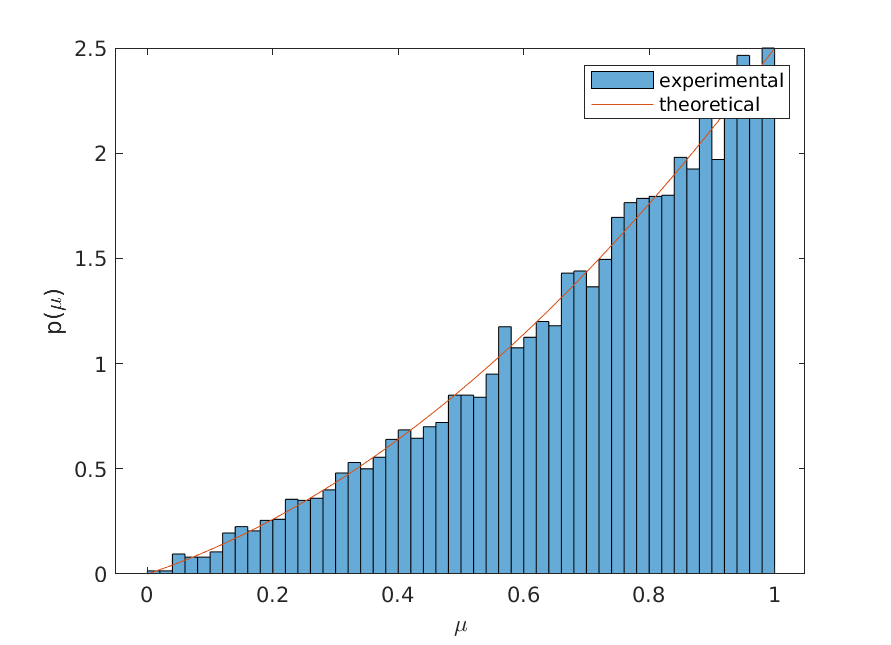
\includegraphics[width=0.7\textwidth]{../../introductory_exercises/P_Cygni_profile_UV_resonance/data/Eddington_accept_reject.png}
\caption{Accept-reject method for Eddington limb darkening}
\end{figure}

\end{enumerate}

Via this link, you can go back to the exercises overview: Section \underline{\ref{Overview_Part_2}}.

\newpage
\subsubsection{Fourth adaptaion: photospheric line-profile}
Challening: Put photospheric line-profile (simple Gaussian) in. What happens? Test on \texttt{xk0=0} (opacity = 0) case.

\begin{itemize}
\item test case number 4 
\item \noindent\fbox{
  \parbox{0.5\textwidth}{This is still to be implemented.}}
\end{itemize}

\newpage
\subsubsection{Convergence analysis}
\label{convergence_analysis}

\paragraph{\underline{Zero opacity}}
The convergence of the Monte Carlo method is tested with the following input parameters

\begin{center}
\centering
{\tabulinesep=1.5mm
\begin{tabu}{|c|c|c|c|}
\hline 
\texttt{kx0} & alpha & beta & \texttt{test\_number} \\
0 & 0 & 1 & 0 \\ \hline
\end{tabu}}
\end{center}

for a varying amount of photons, as shown in Figure \ref{Convergence_Pcyg_kx0_0}. We expect the method to have $\frac{1}{\sqrt{N}}$ convergence, where $N$ is the number of photons. However, the methods strangely seems to have a faster convergence rate. 

\begin{figure}[!htp]
\centering
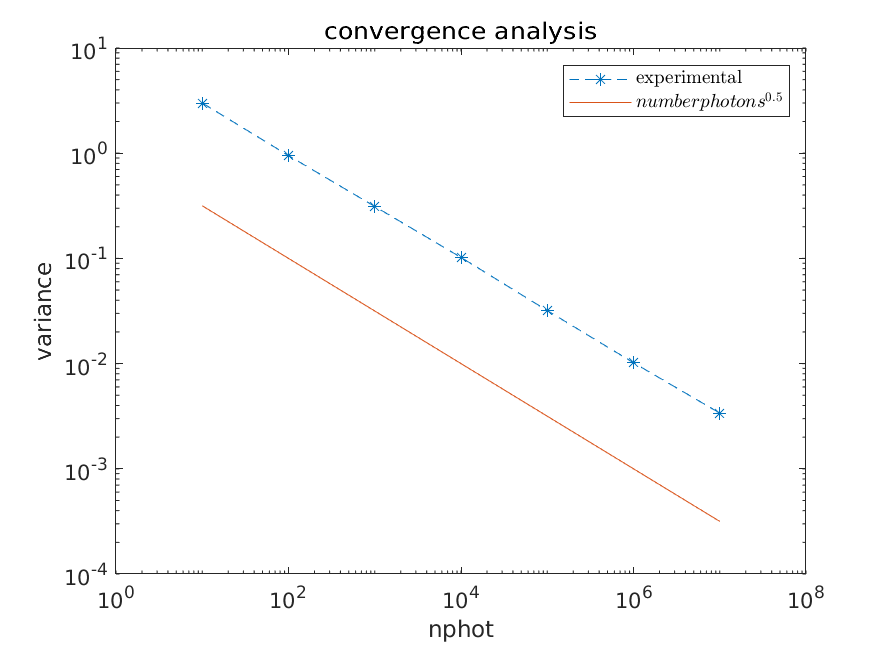
\includegraphics[width=0.5\textwidth]{../../introductory_exercises/P_Cygni_profile_UV_resonance/data/test0_convergence.png}
\caption{Original version of the code: convergence analysis (xk0=0)}
\label{Convergence_Pcyg_kx0_0}
\end{figure}

\paragraph{\underline{Nonzero opacity}} 
The convergence test is set up as follows: different Monte Carlo simulations (with increasing number of photons) are compared to an \textit{expensive} simulation with $10^7$ photons. As can be seen in Figure \ref{Convergence_Pcyg_kx0_100}, the spectrum profile behaves according to a $N^{0.5}$ law.

\begin{figure}[!htp]
\centering
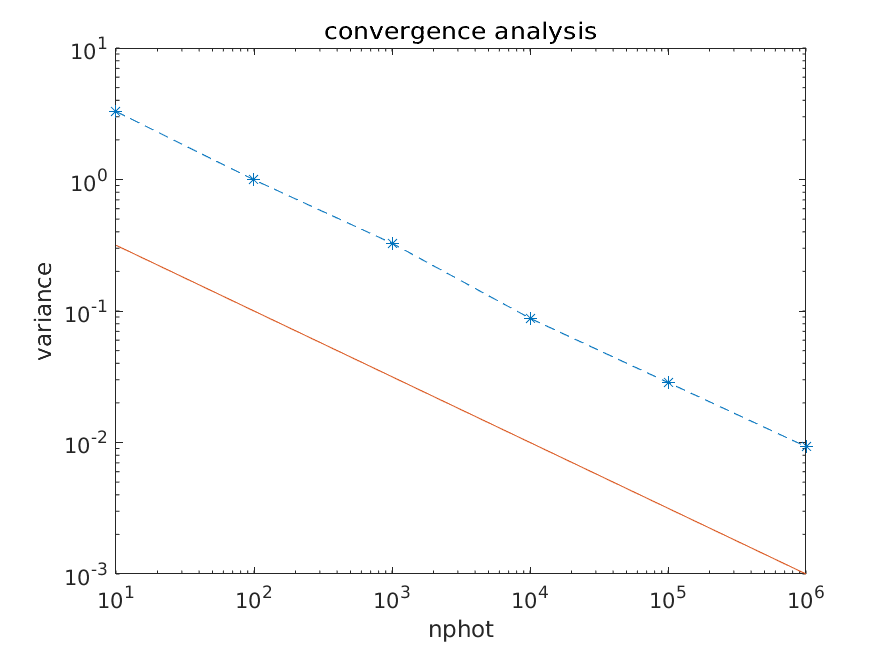
\includegraphics[width=0.5\textwidth]{../../introductory_exercises/P_Cygni_profile_UV_resonance/data/profile_convergence/test0_convergence.png}
\caption{Original version of the code: convergence analysis (xk0=100)}
\label{Convergence_Pcyg_kx0_100}
\end{figure}


Via this link, you can go back to the exercises overview: Section \underline{\ref{Overview_Part_2}}.


\newpage
\subsubsection{Variance reduction experiment}
\label{variance_reduction_experiment}

We will set up the test as follows
\begin{itemize}
\item run the code with \texttt{xk0=100} and number of photons $N=10^7$
\item run the code again for lower number of photons (e.g. $N=10^3$), both with random sampling and pseudo-random sampling
\item compute variance w.r.t. \textit{expensive} simulation and compare
\item \texttt{test\_number = 5}
\end{itemize}


\paragraph{\texttt{xk0=100}}
\begin{figure}[!htp]
\centering
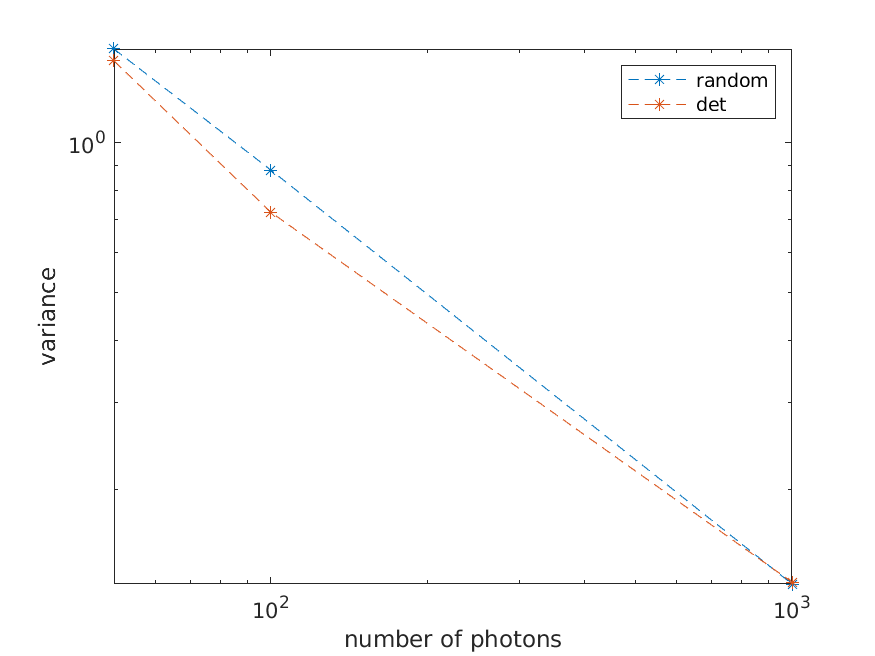
\includegraphics[width=0.65\textwidth]{../../introductory_exercises/P_Cygni_profile_UV_resonance/data/variance_reduction_test.png}
\caption{Original version of the code: convergence analysis (xk0=0)}
\label{variance_reduction_test}
\end{figure}

\paragraph{\texttt{xk0=100}}


\noindent\fbox{
  \parbox{\textwidth}{
Possible improvement: average over different stochastic realizations.}}

\vspace{0.7cm}
Via this link, you can go back to the exercises overview: Section \underline{\ref{Overview_Part_3}}.

\newpage
\subsection{Mathematical description of the problem \\
Looking at literature}
Have a look at \cite{NoebauerUlrichM_2019MCRT}.

\vspace{0.4cm}
Via this link, you can go back to the exercises overview: Section \underline{\ref{Overview_Part_3}}.


\subsection{One more question}
What does this mean? \texttt{xnew=xstart+(v-sign(0.06,xmueou))*xmueou-v*xmuein}

\newpage
\section{Dual spectral line formation}
\label{two_resonance_lines}

\subsubsection{Introduction of second line: theoretical}
\label{second_line}
What happens when you add a line (e.g. \@ $x=0.5=a$)? How would you do that?


\paragraph{Single line}
\begin{center}
\vspace{-0.45cm}
\begin{algorithm}[!htp]
\caption{\texttt{pcyg.f90: one resonance line}}
\label{pcyg_one_line}
\begin{algorithmic}
\For{all photons} 

\begin{enumerate}
\item Release photon with frequency $x$
\item Check if interaction is uberhaupt possible.
\item Solve for distance (radius $r$) of interaction using Sobolev approximation $x_{CMF} = x_{REL} - \mu v(r)$ with $\boxed{x_{CMF} = 0}$ and compute Sobolev optical depth
\item Check whether the photon is scattered:
\end{enumerate}
\If{$\tau_S > -log(\xi)$}
\State Interaction: the photon is scattered. Update the frequency
\Else \State No interaction
\EndIf

\begin{enumerate}
\setcounter{enumi}{3}
\item update the frequency according to the scattering event
\end{enumerate}
	
\EndFor
\State \textbf{end for}
\State collect photons and perform visualisation

\end{algorithmic}
\end{algorithm}
\end{center}

\paragraph{Introduction of second line}
The changes are marked in blue.

\begin{center}
\vspace{-0.45cm}
\begin{algorithm}[!htp]
\caption{\texttt{pcyg.f90: introduction of second resonance line}}
\label{pcyg_one_line}
\begin{algorithmic}
\For{all photons} 

\begin{enumerate}
\item Release photon with frequency $x$
\item Check if interaction is uberhaupt possible.
\item Solve for distance (radius $r$) of interaction using Sobolev approximation $x_{CMF} = x_{REL} - \mu v(r)$ with $\boxed{x_{CMF} = 0}$ and compute Sobolev optical depth 
\item \textcolor{blue}{solve $x_{REF} = x_{CMF} - \mu v(r)$ with $\boxed{x_{CMF} = a}$ for $r_{\text{interaction}}$}
\item \textcolor{blue}{Choose the event corresponding with the lowest value of $r_{\text{interaction}}$}
\item Check whether the photon is scattered:
\end{enumerate}
\If{$\tau_S > -log(\xi)$}
\State Interaction: the photon is scattered. Update the frequency.
\textcolor{blue}{Is there a second scattering event?
\begin{enumerate}[leftmargin=0.6in]
\item Check if interaction is uberhaupt possible.
\item Solve $x_{REF} = x_{CMF} - \mu v(r+ r_{\text{interaction}})$ with $\boxed{x_{CMF} =b}$ where $b$ is the frequency where no scattering has yet found place
\item Check whether the photon is scattered:
\end{enumerate}}
\If{\textcolor{blue}{$\tau_{S,2} > -log(\xi_2)$}}
\State \textcolor{blue}{Second interaction: the photon is scattered once again. Update the frequency.}
\Else \State \textcolor{blue}{No second interaction}
\EndIf

\Else \State no interaction
\EndIf	
\EndFor
\State \textbf{end for}
\State collect photons and perform visualisation
\end{algorithmic}
\end{algorithm}
\end{center}

\newpage
pitfalls yet to solve:
\begin{itemize}
\item root must be bracketed
\end{itemize}


\vspace{0.7cm}
Via this link, you can go back to the exercises overview: Section \underline{\ref{Overview_Part_3}}.

\newpage
\section{Closer look at Monte Carlo simulations}
\label{diffusion_Monte_Carlo_mean_free_path}

\subsection{Random walk (diffusion equation)} A more simple experiment that simulates the diffusion equation (1D random walk) is also set up. The results are shown in Figure \ref{random_walk_N_vs_tau}.
	\begin{figure}[!htp]
	\centering
	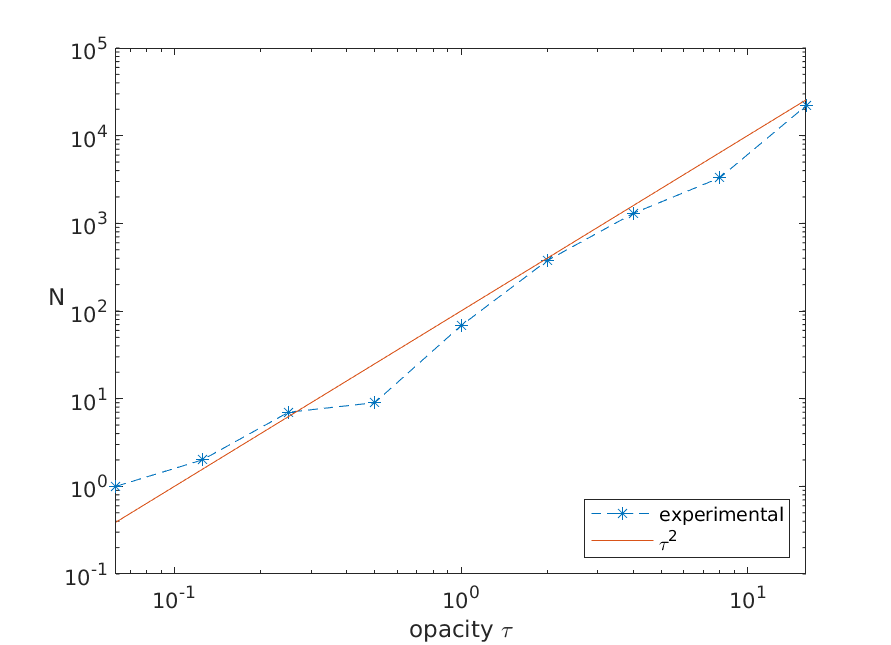
\includegraphics[width=0.5\textwidth]{../../introductory_exercises/limb_darkening/data/diff_N_vs_opacity.png}
	\caption{Number of interactions (scattering events) versus 	opacity, random walk}
	\label{random_walk_N_vs_tau}
	\end{figure}
We observe that $N \sim \tau^2$, as can also be derived from theory.

\begin{itemize}
\item When starting from an initial condition $x_0 = 0$ and 
\begin{equation}
x_N = x_{N-1} \pm l
\end{equation}
we have for the variance that $\braket{x_N}^2 = N l^2$ 
\item If we require a photon to cover a distance $R$ then $N = \frac{R^2}{l^2}$ and
\begin{itemize}
\item the relation between mean-free path $l$ and opacity $\alpha$ is $l = \frac{1}{\alpha}$
\item with $\tau = \int_0^R \alpha ds = \frac{R}{l}$
\end{itemize}
then we have that $N = \tau^2$. This corresponds with the observations in Figure \ref{random_walk_N_vs_tau}.
\end{itemize}


\newpage
\subsection{Limb darkening} We first look at results from the limb darkening program. In Figure \ref{limb_darkening_N_vs_tau}, the number of scattering events is plotted versus the opacity of the medium. 

	\begin{figure}[!htp]
	\centering
	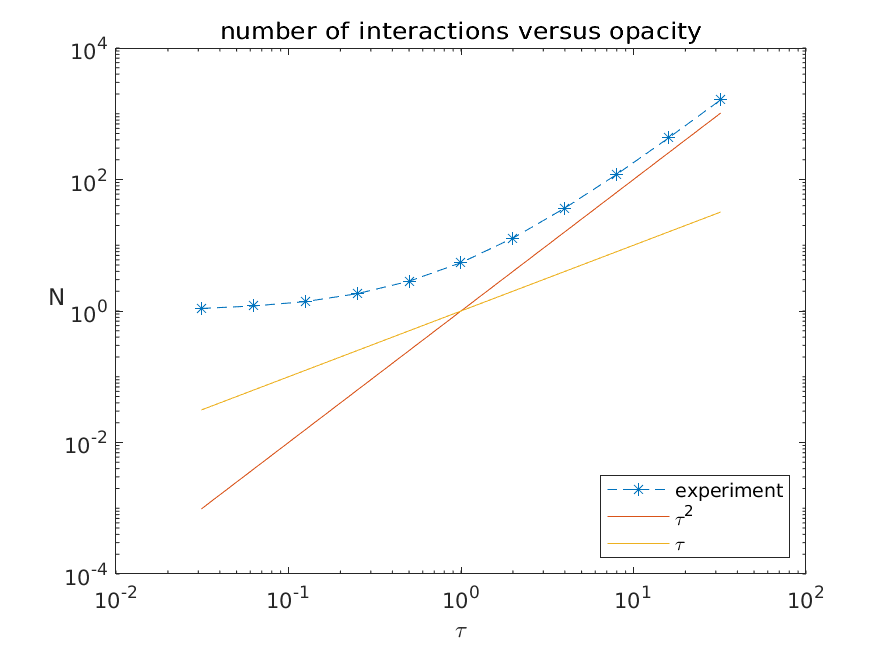
\includegraphics[width=0.5\textwidth]{../../introductory_exercises/limb_darkening/data/N_vs_opacity.png}
	\caption{Number of interactions (scattering events) versus 	opacity, kimb darkening}
	\label{limb_darkening_N_vs_tau}
	\end{figure}

\begin{itemize}
\item For high opacity $\tau \gg 1$ we observe that $N \sim \tau$. \item Bridging regime.
\item For opacity $\tau \ll 1$ we observe that $N \sim 1$: namely the photons travels very far during the first emission event.
\end{itemize}

The splitting scheme from \cite{Dimarco2018} can perfectly be applied to the used Monte Carlo code.

\subsubsection{Eddington-Barbier approximation} 
\begin{equation}
\boxed{J(\tau) = 3H \left( \tau + \frac{2}{3} \right)}
\label{Eddington_Barbier}
\end{equation}
Together with the time-independent radiative transfer equation in a gray (frequency-independent) planar medium:
\begin{equation}
\mu \frac{\partial I(\tau,\mu)}{\partial \tau} = I(\tau,\mu) - J(\tau,\mu)
\end{equation}
that gives
\begin{equation}
\boxed{\mu \frac{\partial I(\tau,\mu)}{\partial \tau} = I(\tau,\mu) - 3H\left(\frac{2}{3}+\tau \right)}
\label{rad_transfer_eq_limb_darkening}
\end{equation}
with the emergent intensity $I(0,\mu)$ as solution of  Equation (\ref{rad_transfer_eq_limb_darkening}). Its solution for $\tau = 0$ equals 
\begin{equation}
I(\tau = 0,\mu) = I_1 \left( \frac{2}{5} + \frac{3 \mu}{5} \right) 
\end{equation}

\subsubsection{Validity of the Eddington-Barbier approximation}
If we assume Equuation (\ref{Eddington_Barbier}) then $I = I_1(a+b\mu)$ thus $J = \frac{1}{2} \int(\tau,\mu) d\mu = \frac{1}{2} \int_0^1 (a+b\mu)d\mu $

\noindent\fbox{
  \parbox{\textwidth}{
  dat ziet er hier niet goed uit }}


\subsubsection{Solving the (integro-differential) radiative transfer equation}
\begin{itemize}
\item the integro-differential equation describing radiative transfer
\begin{equation}
\begin{aligned}
\mu \frac{dI(\tau,\mu)}{d\tau} &= -I(\tau,\mu) + S(\tau)  \\ 
&= -I(\tau,\mu)  + \frac{1}{4\pi} \int I(\tau,\mu) d\Omega
\end{aligned}
\label{RTE_limb_darkening}
\end{equation}
where $\boxed{S(\tau) = \frac{1}{4\pi} \int I(\tau,\mu) d\Omega}$

\item The difficulty resides in the source function

\item Monte Carlo simulation avoids explicit source function: source function implicit in Monte Carlo simulation

\item in the Monte Carlo program, the physics are simulated \textsc{in between two consecutive scattering events} as follows
\begin{equation}
\frac{dI}{dz} = -\alpha I 
\end{equation}
thus $\frac{dI}{I} = -\alpha dz = -\delta \tau$ and $I = I_0 e^{-\delta \tau}$ and thus $\tau$ is sampled according to $\tau = - \log(X_{\text{random}})$
\end{itemize}

\paragraph{Analytical Solution of Equation (\ref{RTE_limb_darkening})}
Ik heb de mosterd gehaald op \cite{Dublin_limb_darkening}.

\begin{equation}
I(0,\mu) = \int_0^{\infty} S(\tau) exp\left( \frac{-\tau}{\mu} \right) d\left( \frac{\tau}{\mu} \right)
\end{equation}

\paragraph{Numerical Solution of Equation (\ref{RTE_limb_darkening})}
First rewrite the equation
\begin{equation}
\begin{aligned}
\mu \frac{dI(\tau,\mu)}{d\tau} 
&= -I(\tau,\mu)  + \frac{1}{4\pi} \int I(\tau,\mu) \sin(\theta) d\theta d\phi 
\\ &= -I(\tau,\mu)  + \frac{1}{4\pi} \int I(\tau,\mu) d\mu d\phi 
\\ &= -I(\tau,\mu)  + \frac{1}{2} \int I(\tau,\mu) d\mu 
\end{aligned}
\end{equation}
Discretization scheme:
\begin{equation}
???
\end{equation}

\noindent\fbox{
  \parbox{\textwidth}{
  If you assume constant opacity then $\tau = \alpha z$
  }}

\newpage
\section{Milic Exercises}
\subsection{Lecture 7}
\begin{enumerate}
\item Derive expressions for the emergent radiation when properties are the following:
\begin{itemize}
\item optically thin slab at all wavelengths
\item wavelength-independent incident radiation
\end{itemize}
Solution: see slide 14?

\item Derive ralations between Einstein coefficients.

\item Calculate electron density in atmosphere from FALC model
\end{enumerate}


\newpage
\section{Mass loss from inhomogeneous hot star winds (Sundqvist)}
\begin{itemize}
\item GOAL: synthesis of UV resonance lines from inhomogeneous 2D winds
\begin{itemize}
\item clumped in density
\item clumped in velocity
\item effects of non-void inter-clump medium
\end{itemize}

\item WIND MODELS
\begin{itemize}
\item symmetry assumptions
\begin{itemize}
\item 1D: spherical symmetry
\item 2D: symmetry in $\Phi$
\end{itemize}

\item models
\begin{enumerate}

\item time-dependent radiation-hydrodynamic from Puls and Owocki (POF)
\begin{itemize}
\item 1D
\item isothermal flow
\item perturbations triggered by photospheric sound waves
\end{itemize}

\item time-dependent radiation-hydrodynamic from Feldmeier (FPP)
\begin{itemize}
\item 1D
\item treatment of energy equation
\item perturbations triggered by photospeheric sound waves or Langevin perturbagions (photospheric turbulence)
\end{itemize}

\item stochastic model, clumped in density
\begin{itemize}
\item smooth winds with $v_{\beta} = (1-b/r)^{\beta}$ with $\beta = 1$
\item clumping factor $f_{cl}$
\end{itemize}

\item stochastic model, clumped in density and in velocity (non-monotonic velocity field)
\begin{itemize}
\item smooth winds with $v_{\beta} = (1-b/r)^{\beta}$ with $\beta = 1$
\item clumping factor $f_{cl}$
\end{itemize}
\end{enumerate}

\end{itemize}

\item RADIATIVE TRANSFER (MC-2D)
\end{itemize}

\newpage
\section{Asymptotic preserving Monte Carlo methods for radiative transfer equation in diffusion limit (Dimarco+ 2018)}
\subsection{Goldstein-Taylor}
\subsection{Radiative transfer}

\newpage
\section{Do not forget}
\begin{itemize}
\item convergence plots
\end{itemize}

\end{document}